\chapter{Resultados} \label{resultado}
Para a primeira etapa do projeto, fizemos a análise espacial para os dados de São Paulo. Por problemas na aplicação que coleta as geocodificações, obtivemos resultados apenas para 3 APIs (TomTom, Mapbox e Here). Abaixo serão apresentados os resultados obtidos.

\section{Distribuição Espacial dos Pontos Geocodificados}
Após a geodificação dos dados, era interessante vizualizar como os pontos geocodificados estavam distribuídos no espaço e o quão diferente era dos pontos ouro. Para isso, foram gerados mapas com a identificação dos pontos para cada uma das APIs.

Não é possível tirar muitas conclusões definitivas apenas com essa visualização, no entanto, é possível observar a densidade dos pontos e identificar que em todas as APIs houve uma maior concentração de dados ouro. Porém em algumas APIs essa concentração é visivelmente menor que a outra. Além disso, pode-se notar que os pontos classificados como "Gold" estão concentrados na região metropolitana de São Paulo, enquanto alguns pontos geocodificados estão localizados fora dessa região, em outras cidades do estado. Essa disparidade provavelmente reflete alguns erros graves de geocodificação, conhecidos como outliers. Esses outliers estão presentes desde mais próximos a região metropolitana do município de São Paulo mas estão também em outros lugares do estado de São Paulo.

Na \ref{fig:mapapontos1} podemos vizualizar a distribuição espacial dos pontos geocodificados pela Mapbox. Nela é possível observar a presença dos outliers citados anteriormente. Porém, são poucos os pontos em que houve essa falha. Portanto considerando apenas essa análise, a API teve resultado satisfatório.

\begin{figure}[h]
  \centering
  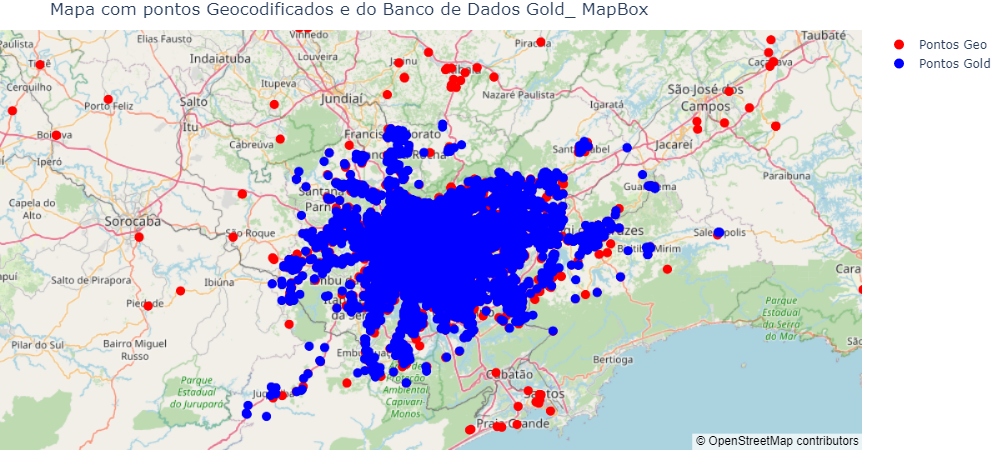
\includegraphics[width=\textwidth]{Figuras/mapapontos1.png}
  \caption{Mapa da Distribuição Espacial dos Pontos da base Gold e Geocodificados pela Mapbox}
  \label{fig:mapapontos1}
\end{figure}

Na \ref{fig:mapapontos2} podemos observar a distribuição espacial dos pontos geocodificados pela Here. Fica claro na imagem que houve uma diminuição significativa dos pontos. O que indica que a resposta da API foi baixa. Com essa quantidade de pontos não é possível tirar conclusões fortes sobre os dados, porém observamos que além da baixa resposta os pontos parecem estar em locais distintos. Esse resultado foi então considerado insatisfatório. Em outro momento, o experimento será repetido para que possamos tirar as conclusões corretas.

\begin{figure}[h]
  \centering
  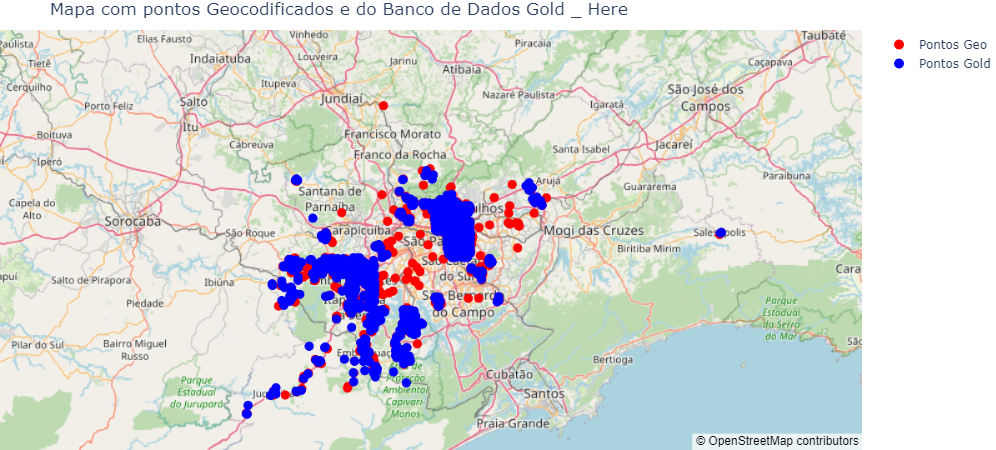
\includegraphics[width=\textwidth]{Figuras/mapapontos2.png}
  \caption{Mapa da Distribuição Espacial dos Pontos da base Gold e Geocodificados pela Here}
  \label{fig:mapapontos2}
\end{figure}

Já a \ref{fig:mapapontos3} mostra a distribuição espacial dos pontos geocodificados pela TomTom. Com esse mapa, é possível observar que a resposta da API foi boa em comparação com os mapas apresentados anteriormente. Também teve alguns outliers e aparentemente esses estão em maior quantidade que na \ref{fig:mapapontos3} e estão mais espaçados geograficamente. Apesar disso, apenas com essa análise, consideramos o resultado satisfatório. 

\begin{figure}[h]
  \centering
  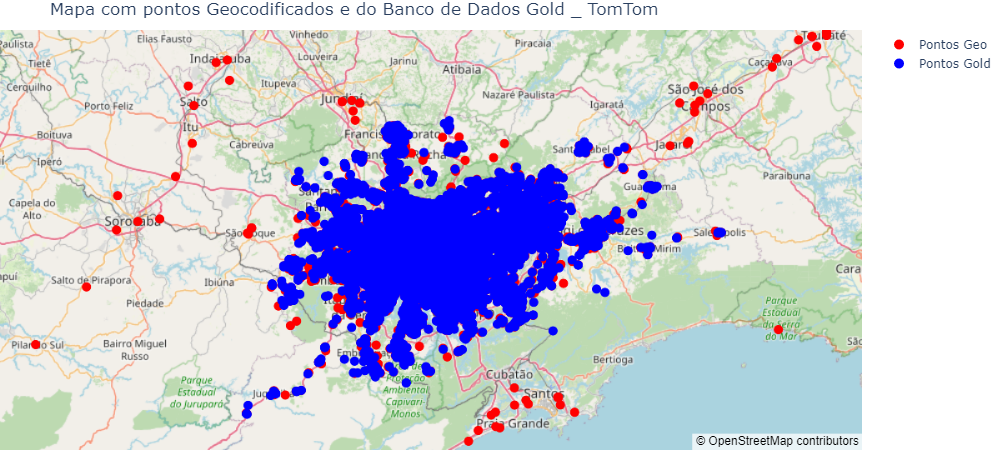
\includegraphics[width=\textwidth]{Figuras/mapapontos3.png}
  \caption{Mapa da Distribuição Espacial dos Pontos da base Gold e Geocodificados pela TomTom}
  \label{fig:mapapontos3}
\end{figure}



\subsection{Metrícas do Erro}
Após essa análise, o erro foi calculado para cada um dos pontos, sendo expresso em quilômetros.

Com essa informação, foram calculadas as métricas mencionadas anteriormente. É notável que a API TomTom obteve a maior taxa de resposta, com um índice superior a 80\%. Além disso, apresentou a melhor média aparada em 5\%. Por outro lado, a API Here obteve um desempenho superior na média tradicional, apesar de possuir uma taxa de resposta muito baixa. De forma geral, esses resultados foram considerados insatisfatórios. Ao longo do relatório, iremos analisar outras questões em detalhes.

\begin{table}
  \centering
  \caption{Métricas de Erro e Resposta}
  \setlength{\tabcolsep}{4pt}
  \begin{tabular}{|c|c|c|c|c|c|c|}
  \hline
  \makecell{API} & \makecell{Média \\(km)} & \makecell{Mediana \\(km)} & \makecell{Desvio \\Padrão (km)} & \makecell{Média \\Aparada (km)}(km) & \makecell{Taxa de \\Resposta (\%)} & \makecell{Taxa de \\Acerto(\%)}\\
  \hline
  Mapbox & 9.7544 & 0.1084 & 46.7664 & 1.8349 & 53.3829 & 30.1903 \\
  Tomtom & 5.0701 & 0.0560 & 35.6215 & 0.2373 & 83.1894 & 9.2051 \\
  Here & 2.2372 & 0.0632 & 13.7984 & 0.4365 & 13.9075 & 9.2051 \\
  \hline
  \end{tabular}
\end{table}

\subsection{Distribuição do Erro}
Em seguida, tentamos analisar a distribuição do erro para cada uma das GeoAPIs. Para isso, utilizamos histogramas de erro individualmente para cada API e combinando todas elas. No entanto, devido à presença de alguns erros exorbitantes, esses histogramas não eram muito representativos, pois a maior parte do erro se concentrava entre 0 km e 50 km. Diante disso, decidimos realizar um corte nos dados, limitando o erro em 0.5 km ou 500 metros. Em seguida, repetimos o processo, agora gerando um único histograma que representa a distribuição do erro para todas as APIs em conjunto.

Com base nos histogramas, pudemos observar que a maioria dos erros está concentrada entre 0 e 200 metros. Levando em consideração nossas pesquisas, consideramos um erro aceitável de até 150 metros, o que corresponde aproximadamente a um quarteirão. Portanto, com base apenas na análise da distribuição de erros, todas as APIs apresentam resultados satisfatórios.

\begin{figure}[h]
  \centering
  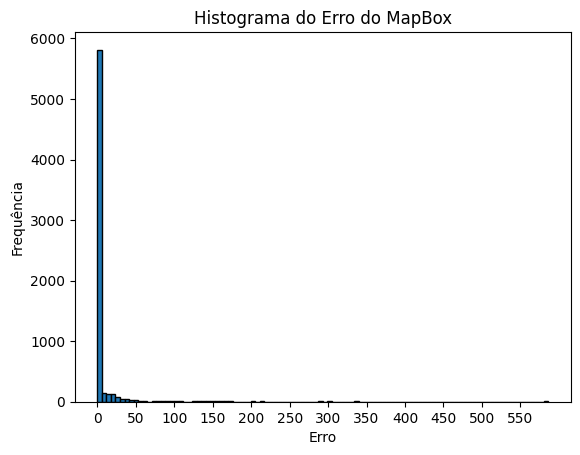
\includegraphics[width=\textwidth]{Figuras/hist1.png}
  \caption{Histograma do erro calculado com os pontos da Mapbox}
  \label{fig:hist1}
\end{figure}

\begin{figure}[h]
  \centering
  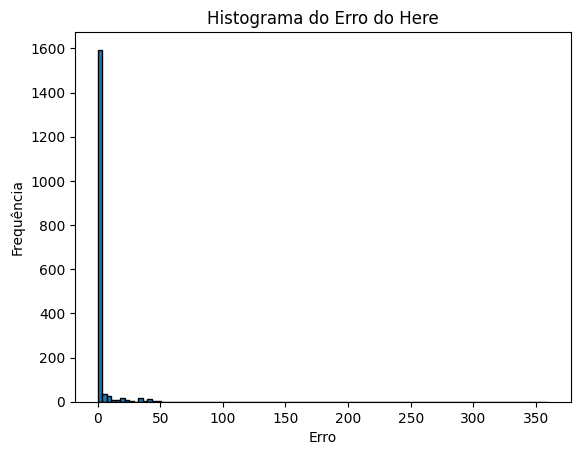
\includegraphics[width=\textwidth]{Figuras/hist2.png}
  \caption{Histograma do erro calculado com os pontos da Here}
  \label{fig:hist2}
\end{figure}

\begin{figure}[h]
  \centering
  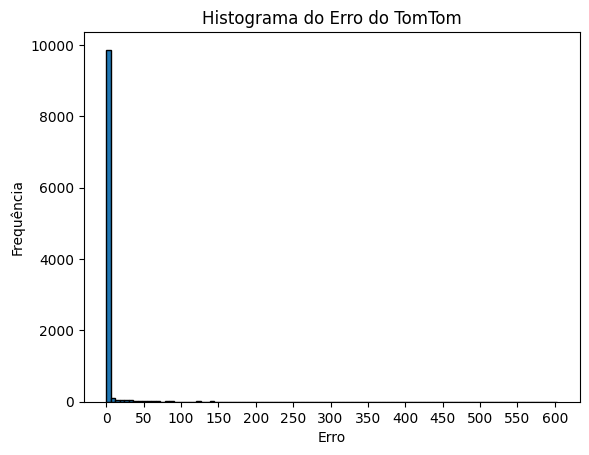
\includegraphics[width=\textwidth]{Figuras/hist3.png}
  \caption{Histograma do erro calculado com os pontos da TomTom}
  \label{fig:hist3}
\end{figure}

\begin{figure}[h]
  \centering
  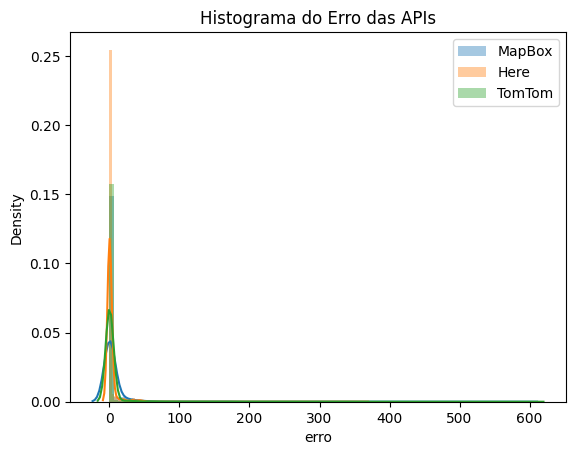
\includegraphics[width=\textwidth]{Figuras/hist4.png}
  \caption{Histograma comparativo do erro das APIs}
  \label{fig:hist4}
\end{figure}

\begin{figure}[h]
  \centering
  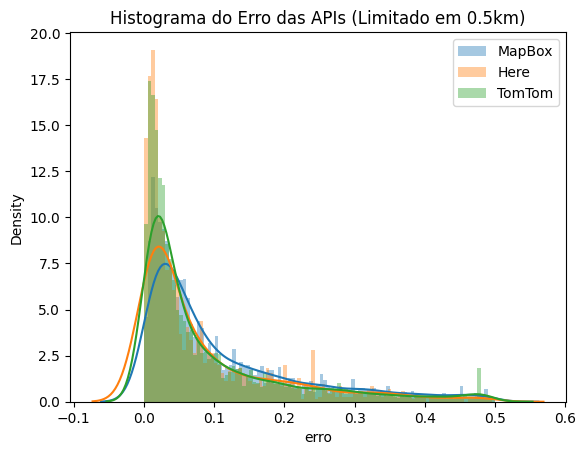
\includegraphics[width=\textwidth]{Figuras/hist5.png}
  \caption{Histograma comparativo do erro das APIs com limitação em 500 metros}
  \label{fig:hist5}
\end{figure}

\subsection{Distribuição Espacial do Erro}
Além disso, realizamos uma análise adicional para visualizar como esse erro se comporta no espaço. Para isso, criamos mapas de altitude, onde o erro foi utilizado como medida de altitude. Nessa representação, cores mais próximas do vermelho indicam erros mais altos, enquanto cores mais próximas do azul escuro indicam erros mais baixos. Também plotamos os pontos geocodificados no mapa para avaliar a representatividade das cores. Dessa forma, pudemos verificar se uma determinada área apresenta muitos pontos geocodificados ou se há poucos pontos com erros grandes.

Ao analisar os resultados, observamos que a maioria do mapa apresenta erros menores que 34 km, conforme esperado. No entanto, identificamos alguns pontos com erros grandes, que serão avaliados individualmente posteriormente. É importante ressaltar que encontramos uma limitação devido à presença de erros exorbitantes, ou outliers, o que restringe nossa capacidade de tirar conclusões significativas. Para obter uma melhor compreensão do contraste e da distribuição geográfica do erro, planejamos repetir o experimento realizando um corte em 34 km.

É válido destacar que o mapa é interativo no projeto original, permitindo uma visualização mais detalhada das informações apresentadas.

\begin{figure}[h]
  \centering
  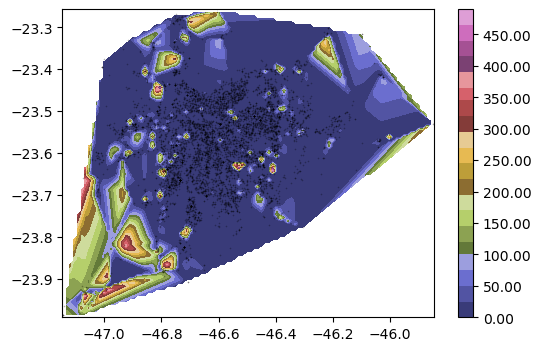
\includegraphics[width=\textwidth]{Figuras/graficoAltPontosMapbox.png}
  \caption{Gráfico de altitude do erro (km) da geocodificação da Mapbox.}
  \label{fig:grafAltM}
\end{figure}

\begin{figure}[h]
  \centering
  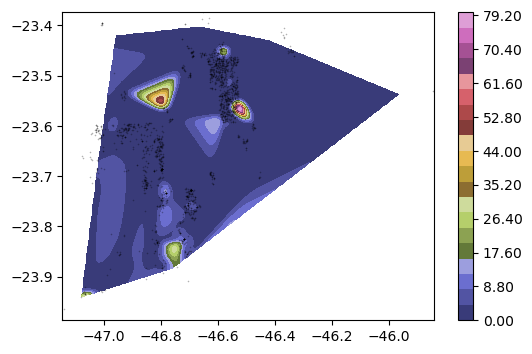
\includegraphics[width=\textwidth]{Figuras/graficoAltPontosHere.png}
  \caption{Gráfico de altitude do erro (km) da geocodificação da Here.}
  \label{fig:grafAltH}
\end{figure}

\begin{figure}[h]
  \centering
  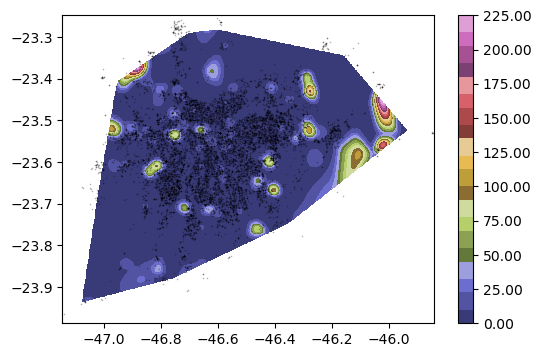
\includegraphics[width=\textwidth]{Figuras/graficoAltPontosTomtom.png}
  \caption{Gráfico de altitude do erro (km) da geocodificação da TomTom.}
  \label{fig:grafAltT}
\end{figure}